\documentclass[a4paper,12pt]{article}
%\usepackage[utf8x]{inputenc}
\usepackage[utf8]{inputenc}
%\usepackage{lipsum}
\usepackage{amsmath,amsthm,mathrsfs}
\usepackage[english]{babel}
\usepackage{textcomp}
%\usepackage[T1]{fontenc}
\usepackage{graphicx,wrapfig}
\usepackage{amssymb}

\newcommand\norm[1]{\left\lVert#1\right\rVert}
\usepackage{calc}
\usepackage{rotating}
\usepackage[usenames,dvipsnames]{color}
\usepackage{fancyhdr}
%\usepackage{subfigure}
\usepackage{hyperref}
\usepackage{longtable}
\usepackage{svg}
\usepackage{float}
\usepackage{rotating}
\usepackage[usenames,dvipsnames]{color}
\usepackage{fancyhdr}
%\usepackage{subfigure} 
\usepackage[english]{babel}
\usepackage[backend=bibtex,
style=numeric,
bibencoding=ascii,
sorting=none
%style=alphabetic
%style=reading
]{biblatex}
\usepackage{hyperref}
\addbibresource{prop_ref}
\usepackage[a4paper, margin=1.5in]{geometry}
\usepackage{pifont}
\usepackage{xcolor}
\usepackage{dirtytalk}
\hypersetup{
    colorlinks,
    linkcolor={red!50!black},
    citecolor={blue!50!black},
    urlcolor={blue!80!black}
}
\graphicspath{{images/}}
%\usepackage{times}
%\usepackage[scaled=0.8]{beramono}
 \renewcommand{\familydefault}{\rmdefault}
\begin{document}

\begin{titlepage}
\pagenumbering{gobble}
\begin{center}

 
%	\noindent\rule[0.5ex]{\linewidth}{4pt}
%  

  \vskip.1in
  \textbf{\Large Information-Performance Tradeoffs in Control}  \vskip.7in
  \vskip.7in
%\noindent\rule[0.5ex]{\linewidth}{4pt}
	\begin{center}\textit{\small{Project proposal document}} \\
	\textit{\small{for Visiting Undergraduate Research Program}}
	
	\textit{by}
	\vskip.3in
	
	\textbf{\normalsize AYUSH PANDEY}\\
	\end{center}
\end{center}
%\vskip1.3in
%\begin{minipage}[t]{7cm}
%\flushleft
%\textsc{Author:}
%%
%Ayush Pandey \\12IE32001\\ IIT Kharagpur \\
%\end{minipage}
%\hfill
%\begin{minipage}[t]{7cm}
%\flushright
%\textsc{Supervisor:}
%
%Dr. Sourav Patra \\IIT Kharagpur
%\end{minipage}
%\vskip1.2in
\vskip.9in
\vskip.9in
\vskip.3in

\begin{flushleft}
\vskip.1in
Mentor :\textbf{ Dr. Victoria Kostina}
\\
Electrical Engineering
\\
California Institute of Technology\\
May 2016
\end{flushleft}


\end{titlepage}


\section{Introduction}
\label{intro}
	Over the past few decades the fields of communication and control have been developed extensively to support the emerging needs of the society such as higher speed internet, better telephone communication networks, wireless access to devices over Internet of Things (IoT), reliable long distance satellite communication, home automation and many other related fields. Communication theory is mainly concerned with the transmission of information from one point to another reliably without putting much concern over what is done with that information once it is transmitted. Control theory mainly deals with the feedback of information in order to achieve better performing systems, which are not prone to disturbances, noises and other process variations. Control systems without physical inter-connection between its subsystems for eg. when signals between sensors and/or controllers and the plant are transmitted over communication channels are called networked control systems. Networked control finds wide applications but also poses newer challenges which control theory doesn't deal with. There are various additional constraints that have to be kept in mind while designing the control system. For eg. noise in the communication channels, quantization effects for digital communication devices, time delays, packet losses etc. \\
    Optimal control design deals with optimization (often minimization) of a performance index subject to system state equation constraints to obtain an optimal control law. When the performance index is a quadratic function of states and control input (for a deterministic system), this optimal control design is commonly referred to as the Linear Quadratic Regulator (LQR) control problem. The LQR control gives good robustness features. A big disadvantage with LQR design is that it requires measurement of all the states. Usually in physical systems, this is not possible. Even when it is possible to measure all the states, it is usually very expensive. To overcome this problem, the states are computationally estimated and then the estimated states are used to design the control. The estimation based control poses its own challenges. The estimation of states for physical systems is seldom free of noise. This inaccuracy in estimation results in deterioration of the performance.  It is intuitively understood that the better the observation accuracy, the better the system performance would be. This project aims to deal with the tradeoff between estimation (observation) accuracy and performance in networked control systems. \\
   In this document, we will first cover the literature in brief and some well known theoretical concepts. We will end with proposing the major objectives for the project.
   \\
\section{Background and Literature Review}
We are interested in the tradeoff between observation accuracy and minimum achievable performance index for a networked control system facing constraints such as quantized estimation (limited data rate of communication) and multiplicative uncertainity in control signal or system state(s). These form the background of the work that would be done in this project. Also, the control scheme that we would be dealing with the most in this project is the Linear Quadratic Gaussian (LQG) control. We start by going over the well-known concepts of partially observed LQG problem.
	\subsection{Classical Partially Observed LQG Problem}
	For a stochastic system, the LQG control scheme estimates the states from the available outputs. Using this estimation of states a controller is designed such that a quadratic performance index is minimized. Consider a discrete time stochastic system, the state equation can be written as
	\begin{align}
	x_{t+1} &= A_{t}x_{t}+ B_{t}u_{t} + w_{t}\\
	\intertext{The output equation is}
	y_{t}&=C_{t}x_{t}+v_{t}
	\end{align}
	where $w_{t}$ and $v_{t}$ are assumed to be zero mean Gaussian noises with covariances $W_{t}$ and $V_{t}$ in process and measurement respectively. For states $x_{t} \in \mathbb{R}^{n \times 1}$, inputs $u_{t} \in \mathbb{R}^{k \times 1}$ and outputs $y_{t} \in \mathbb{R}^{p \times 1}$ we have, the stochastic state transition matrix $A_{t} \in \mathbb{R}^{n \times n}$, the stochastic control multipliers, $B_{t} \in \mathbb{R}^{n \times k}$ and the stochastic output multipliers, $C_{t} \in \mathbb{R}^{p \times n}$. We also assume that the initial value of the state $x$, $x_{0}$ is known and that $w,v$ and $x_{0}$ are all independent of each other. The system is stationary which ensures that the mean and covariances will not change with time. The following block diagram representation gives a clearer picture of LQG control.
	\begin{figure}[H]

			  \centering
%			  \includesvg[width=1.0\textwidth]{block2}
%			  \def\svgscale{5.5}
%			  \tiny{
%			  \input{ulft.pdf_tex}}
			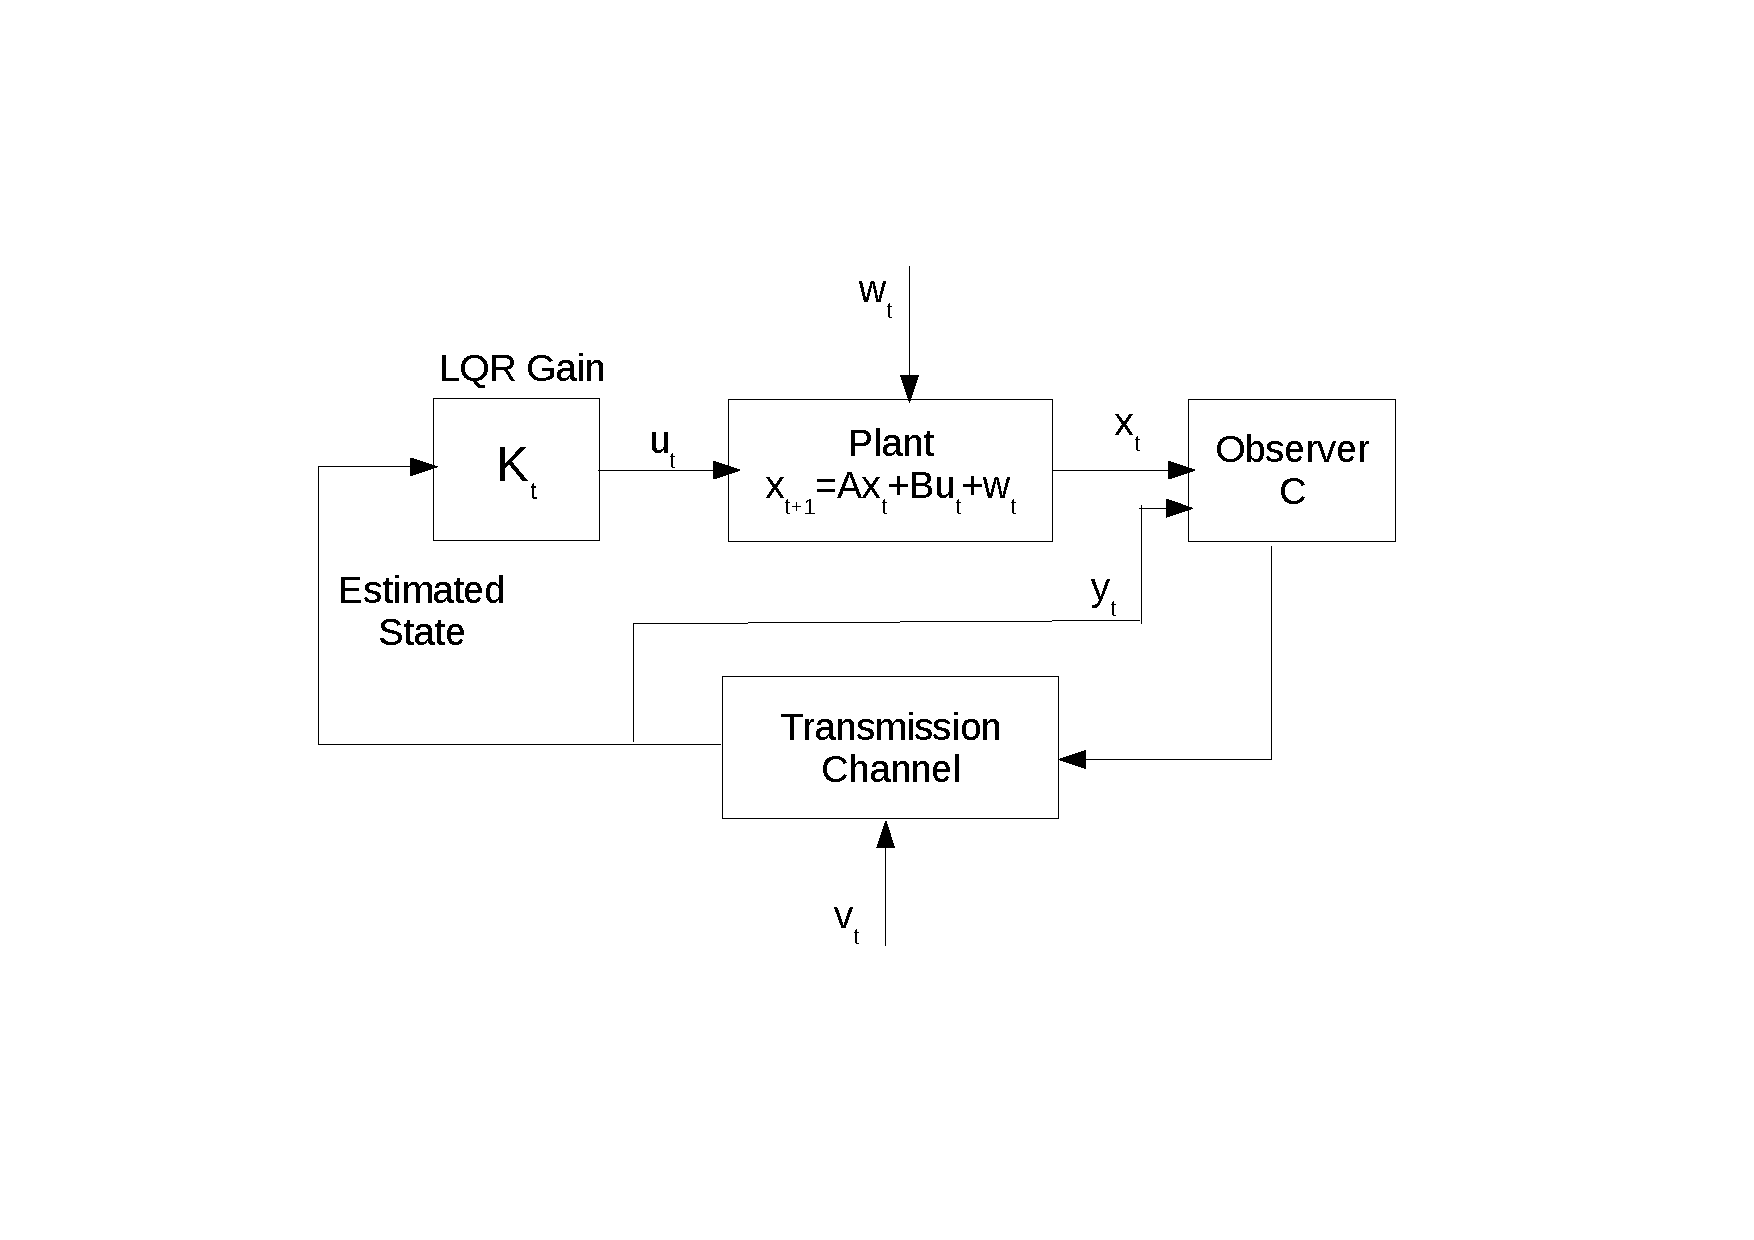
\includegraphics[scale=0.5]{lqg_block}
			  \caption{Representative Block Diagram of Classical Partially Observed LQG Control}
			 \label{lqg}
		\end{figure}	
	
	Our aim is to find a control law $u_{t}$ so that the following performance index is minimized, where $Q \geq 0$ is the state weighting matrix and $R > 0$ is the control weight matrix. 
	\begin{align}
		J(\cdot)&=E\left(\sum\limits_{t=0}^{N-1} \left(x_{t}^{T}Qx_{t} + u_{t}^{T}Ru_{t}\right) + x_{N}^{T}Qx_{N} \right)\\
	\intertext{The control law is given by}
	\label{controleq}
	u_{t}&=K_{t}E[x_{t}|y_{1},y_{2},...,y_{t}]
	\end{align}
	 where $K_{t}$ is the LQR gain and $E[x_{t}|y_{1},y_{2},...,y_{t}]$ is the minimum mean square error estimate of $x_{t}$ given that all past output measurements are available. As we can see in Eq.(\ref{controleq}), the estimate of the state is used for control and not the original states. It can be proved that the calculation of the LQR gain $K_{t}$ and the MMSE estimate of the state using Kalman Filter can be performed independent of each other \cite{book}. 
	\subsection{Quantization Constraints in Networked Control Systems}
	As mentioned in the previous section, Gaussian noises in the plant and measurement might not be the only constraints. For eg. if in Fig.(\ref{lqg}) the observer data is transmitted via a digital communication channel to the controller. Other than the additive Gaussian noise $v_{t}$, the control performance would also be dependent on the data rate at which the communication is done. The limitation on this feedback data rate affects the system performance. Hence, there exists a tradeoff between communication rate and optimal performance. \\
	For a noiseless scalar plant with parameter $|a|>1$, \cite{quantpaper} shows that the minimum data rate required to keep the plant bounded is $\log_{2}|a|$ bits per sample. This is known as the Data Rate Theorem. Similar results have been dervied for linear state-space systems which we are concerned with in this project. The reader is referred to \cite{quantoverview} and references therein for further details. \\
	
	\subsection{Multiplicative Uncertainty in Networked Control Systems}
	Among various constraints in a networked control system such as time delays, data rate constraints, packet loss etc. is the parameter uncertainty constraint. The robust control techniques aim to deal with uncertain plant parameters and it is a very well researched topic (\cite{robust1}, \cite{robust2}). Often, this parametric uncertainty takes a form of multiplicative uncertainty in either the control signal or the states.  \\
	From the control perspective, various techniques have been proposed to design controllers for systems with multiplicative uncertainty. Convex optimization based techniques have also been proposed using linear matrix inequality (LMI) techniques for control design \cite{lmi}. An uncertainty threshold principle has been proposed in \cite{uncthres} which provides an explicit threshold on the uncertainties that can be tolerated in the systems with multiplicative uncertainties. An example of multiplicative uncertainty in a control system is explained using the following block diagram. The system shown below has multiplicative uncertainty in its states.
		\begin{figure}[H]

			  \centering
%			  \includesvg[width=1.0\textwidth]{block2}
%			  \def\svgscale{5.5}
%			  \tiny{
%			  \input{ulft.pdf_tex}}
			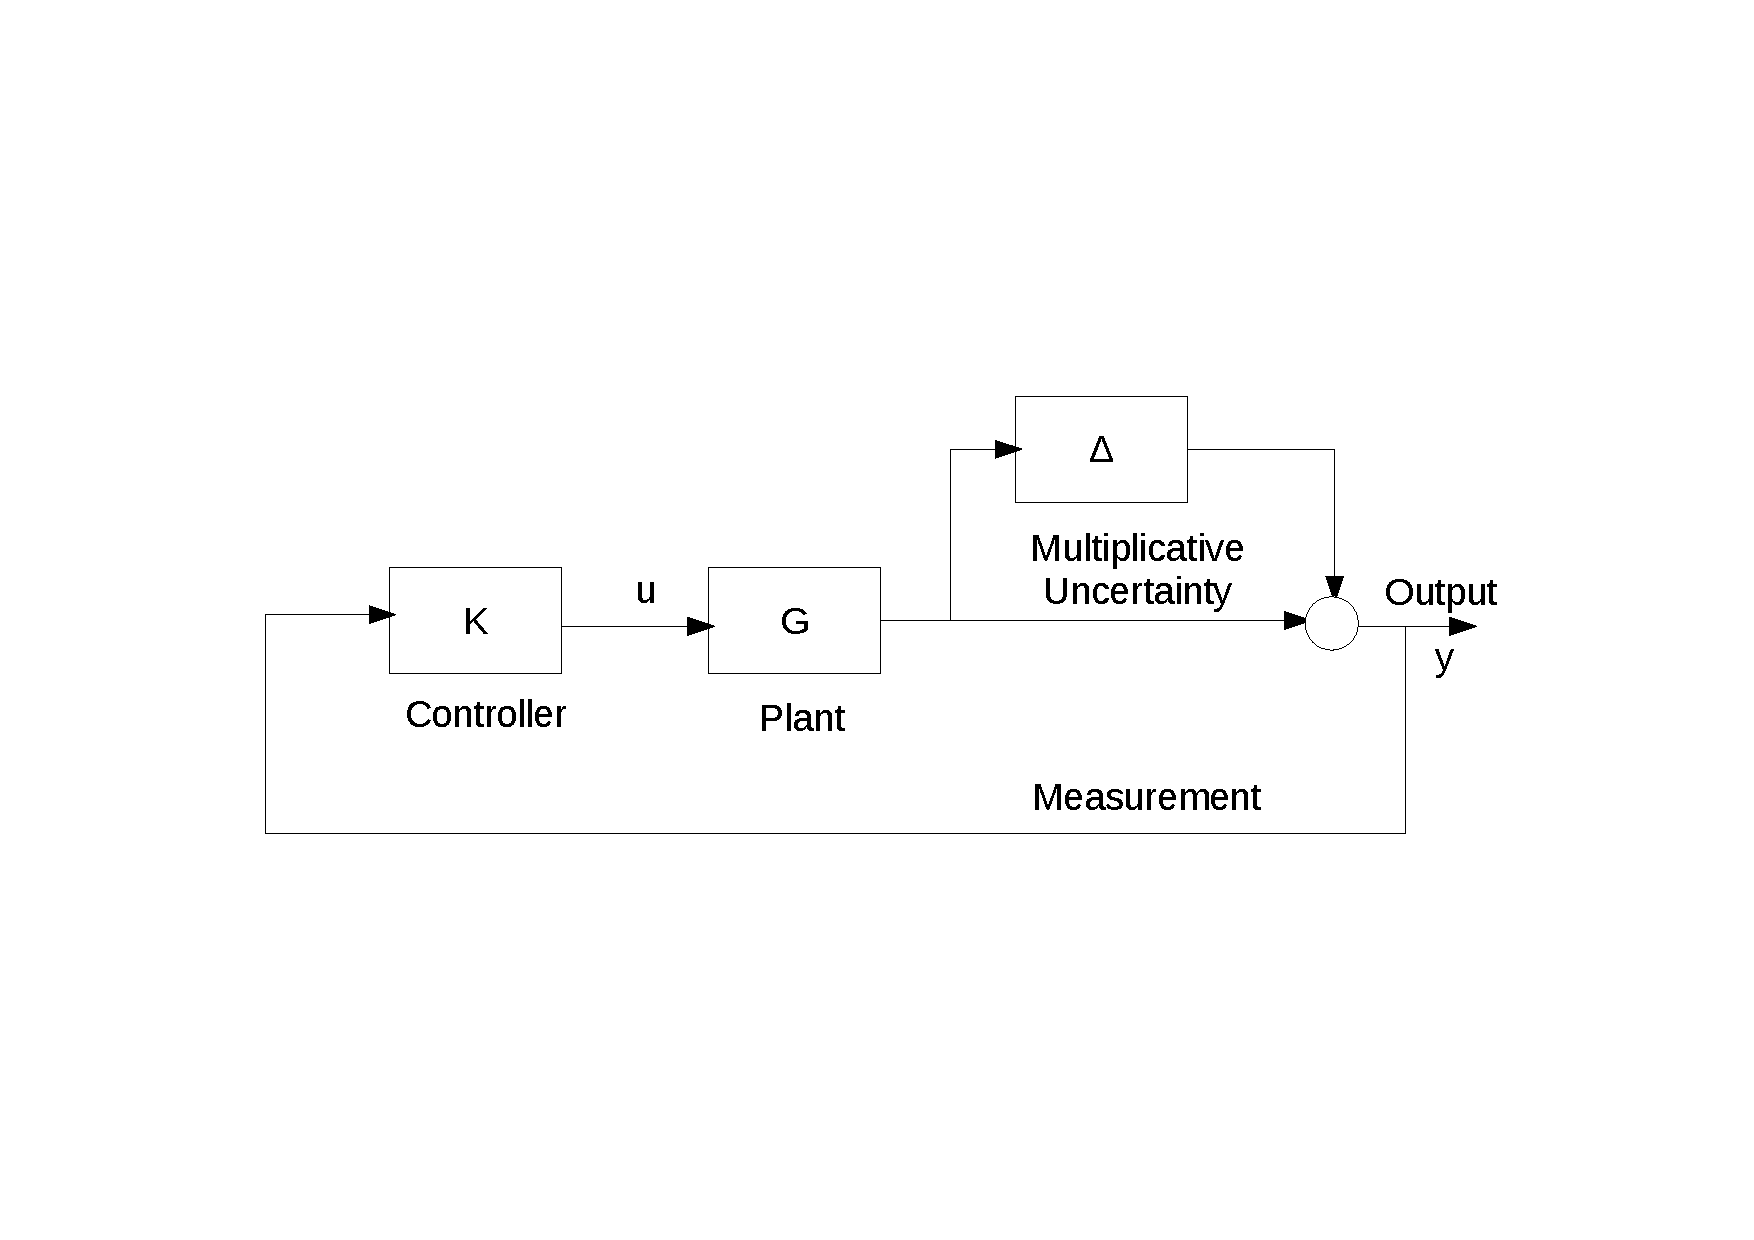
\includegraphics[scale=0.5]{mult}
			  \caption{Multiplicative Uncertainty}
			 \label{mult}
		\end{figure}	
		The uncertain parameter is $\Delta$ which changes the plant transfer function effectively by a factor of $(1+\Delta)$. From Fig.(\ref{mult}) we have, the uncertain plant transfer function, $G_{u}=G(1+\Delta)$, which is a multiplicative uncertainty in the states of the process.\\
		The presence of such multiplicative uncertainties also affects the system performance. The tradeoff between the magnitude of such uncertainties present in the system and the observation accuracy that can be achieved would be of interest to us in this project. Some important results have been given in \cite{mult_thesis}.
\section{Objectives}
For a given stochastic scalar system,
\begin{align}
X_{t+1} &= A_{t}X_{t} + BU_{t} \\ 
\label{outputeq}
Y_{t} &= CX_{t} + W_{t}
\end{align}
where $X_{t+1}$ is the state being estimated from measurements $Y_{t}$. For this stochastic system, $A_{t}$ is a random variable with known distribution and $W$ is the noise in measurement.\\
%add details about w,b,etc.

The project objectives with respect to this scalar system can be expressed in brief as follows:
\begin{enumerate}
\item As described in Section(\ref{intro}), the controller observes $Y_{t}$ and this is used to estimate the states. Under this observation, we would aim to find out the minimum $\underset{t \to \infty}\lim E[{X_{t}^2}]$ achievable in the limit.
\item To improve the estimation accuracy (and hence the performance) we may be interested to estimate the state $X_{t+1}$ by making $n$ measurements $Y_{t_{1}}, Y_{t_{2}}, ... Y_{t_{n}}$ of the output. From Eq.(\ref{outputeq}), we then have,
\begin{equation}
Y_{t_{i}} = CX_{t} + W_{t_{i}} 
\end{equation}
for $i=1,2,..., n$ and where $W_{t_{i}}$ are i.i.d. noise in the measurement.
Clearly, the more observations we make the better the controller’s knowledge of the system state is. However, the measurements can be expensive. So, this project aims to study the tradeoff between the number of observations $n$ and the minimum attainable mean square estimate $\underset{t \to \infty}\lim E[{X_{t}^{2}}]$.
\end{enumerate}
\section{Approach and Timeline}
Initially, some more time would be spent on the literature related to the work in this project. The knowledge of linear quadratic control theory (LQR and LQG control), Riccati equations and their solutions in MATLAB would be very helpful in carrying out the research work on this project successfully and in the given period of time. For the first few weeks, after the literature has been reviewed completely, we would aim to draw out extensions from the existing theory on the tradeoff between the MMSE estimate of the states and the observation accuracy for a simple scalar stochastic system. Once this is done, the case where $n$ measurements are made would be studied and its effect on improvement in performance would be demonstrated. Proficiency with MATLAB programming would be an added advantage in completing this project in the given time. Some of my previous codes written using MATLAB's Robust Control Toolbox, Convex Optimization Toolbox, Control Systems Toolobx and Digital Signal Processing Toolbox are available at \cite{git_rct} and \cite{git_dac} respectively. Also, a repository of all future codes for this project is available at \cite{git}. It would also have codes for progress reports and project proposal, including all images and diagrams.

\printbibliography
     
\end{document} % The document ends here
